\documentclass[12pt,a4paper,english,twoside]{book}
\usepackage[german,english]{babel}
\usepackage[T1]{fontenc} 
\usepackage[latin1]{inputenc}
\usepackage{amsfonts}
\usepackage{amsmath}
\usepackage{latexsym}
\usepackage{amssymb}
\usepackage{epsfig}
\usepackage{moreverb}
\usepackage{rotating}
\usepackage{enumerate}
\usepackage{graphics, graphicx,wrapfig}
\usepackage{fancybox}
\usepackage{picinpar,varioref,floatflt}
\usepackage{ae}
\usepackage{longtable}
\usepackage{textcomp}
\usepackage{float}
\usepackage{url}
\usepackage{unizhdt}
\usepackage[graphicx]{realboxes}

%%%%%%%%%%%%%%%%%%%%%%%%%%%%%%%%%%%%%%%%%%%%%%%%%%

% Define the language of the diploma thesis
\selectlanguage{english}
%\selectlanguage{german}

\pagestyle{headings}

\begin{document}

%%%%%%%%%%%%%%%%%%%%%%%%%%%%%%%%%%%%%%%%%%%%%%%%%%

% Define the author printed on the cover page
\author{Author}
% Define the city and country of the author
\authorcity{City, Country}
% Define the student ID (Matrikelnummer)
\studentid{00-711-999}
% Define the title with optional subtitle
\title{You never saw it comming}
% Define the supervisors
\supervisors{Thomas Grübl}
% Define the submission date
\submissiondate{September 11, 2024}

%%%%%%%%%%%%%%%%%%%%%%%%%%%%%%%%%%%%%%%%%%%%%%%%%%

% Make the title page
\maketitle

% Make the imprint on the back of the cover page
\makeimprint


\pagenumbering{roman}

% Include the files of the diploma thesis
%\cleardoublepage
\chapter*{Declaration of Independence}
\addcontentsline{toc}{chapter}{Declaration of Independence}
I hereby declare that I have composed this work independently and without the use of any aids other than those declared (including generative AI such as ChatGPT). I am aware that I take full responsibility for the scientific character of the submitted text myself, even if AI aids were used and declared (after written confirmation by the supervising professor). All passages taken verbatim or in sense from published or unpublished writings are identified as such. The work has not yet been submitted in the same or similar form or in excerpts as part of another examination.

\vspace{2cm}

Zürich, \hspace{5cm} \hrulefill \\
\hspace*{6.4cm} Signature of student

\chapter*{Kurzfassung}
\addcontentsline{toc}{chapter}{Kurzfassung}
\selectlanguage{german}

Das USB-Protokoll implementiert keine Authentifizierungsmassnahmen f\"ur USB-Peripherieger\"ate. Das erm\"oglicht die Imitation von Eingabeger\"aten (Human Interface Devices) und erlaubt es jeglichen USB-Ger\"aten vorzugeben, ein solches Eingabeger\"at zu sein und dem Computer Befehle zu erteilen. Solche Attacken werden HID-Imitationsangriffe genannt und haben das Potenzial, grossen Schaden anzurichten. Sogenannte BadUSB k\"onnen frei Befehle an Computer senden, wie es auch ein Mensch mit physischem Zugriff k\"onnte, allerdings mit dem Vorteil \"ubermenschlicher Geschwindigkeit, erm\"oglicht durch die eingebauten Mikrocontroller. Ihr gr\"osster Nachteil jedoch sind die fehlenden R\"uckmeldungen, um einsch\"atzen zu k\"onnen, ob die abgegebenen Befehle erfolgreich waren.

Diese Arbeit erkundet die Geschichte solcher Angriffe sowie die Evolution der Massnahmen gegen sie. Zudem setzt sie einen Schwerpunkt auf ein spezifisches BadUSB: das O.MG-Kabel. Sie analysiert die bestehenden Angriffsskripte, die \"uber die offizielle O.MG GitHub-Datenbank verf\"ugbar sind, und gleicht sie mit den Methoden ab, die im MITRE ATT\&CK Framework gelistet sind. Zu einigen unter- oder nicht repr\"asentierten Methoden werden anschliessend sieben neue Angriffe beschrieben und entwickelt. Zus\"atzlich wird der Aufbau und die Implementierung eines Verteidigungsprogramms detailliert beschrieben, das einen neuartigen Ansatz zur Erkennung von O.MG-Ger\"aten aufgrund ihrer USB-Registrierungsmuster beinhaltet. Weiterhin besteht es aus einem Ratenbegrenzer mit zwei Modi: einer Analyse der Zeitabst\"ande zwischen Tastendr\"ucken und einer Analyse der Anzahl der Tastendr\"ucke in einer gesetzten Zeitspanne. Sobald verd\"achtige Aktivit\"at bemerkt wird, trennt das Programm die Verbindung.

Diese Implementationen werden anschliessend evaluiert. Daf\"ur werden die Angriffsskripte auf drei verschiedenen Ger\"aten ausgef\"uhrt und aufgrund ihres Erfolgs beurteilt. Sie wurden ebenfalls gegen das Verteidigungsprogramm getestet, um herauszufinden, wie schnell dieses sie unterbrechen w\"urde.

Es wurde festgestellt, dass einige Skripte flexibler und weniger anf\"allig f\"ur unvorhergesehene Hindernisse sind und daher weniger Anpassungen brauchen. Zudem wurde festgestellt, dass die Registrierungsmusteranalyse sowie der Ratenbegrenzer zuverl\"assig Angriffe erkennen und abbrechen. Die effizienteste Konfiguration f\"ur die Analyse der Zeitabst\"ande ist ein Schnitt von 8 Millisekunden \"uber drei Tastendr\"ucke, w\"ahrend es f\"ur die Zeitfensteranalyse zwei Tastendr\"ucke in einer Zeitspanne von 75 Millisekunden ist.

\chapter*{Abstract}
\addcontentsline{toc}{chapter}{Abstract}

\selectlanguage{english}

The USB protocol does not implement authentication measures for USB peripheral devices. This leaves room for Human Interface Device Spoofing, specifically for USB
devices pretending to be HID and injecting commands to a host. Those attacks are called
HID spoofing attacks and have the potential to wreak havoc on a target computer. Such a
BadUSB has all the capabilities of a human with physical access to the device’s HID, but
with the added advantage of superhuman input speeds provided by its microcontrollers.
However, its main limitation is the lack of feedback mechanisms to assess the outcomes
of its actions. 

This thesis explores the history of such attacks as well as the history of
countermeasures against them. Additionally, it focuses on one commercially available BadUSB: the O.MG cable. It analyses existing attack payloads on the official O.MG
GitHub repository, comparing them to the MITRE ATT\&CK framework and supplementing it with seven new ones. Furthermore, the architecture and implementation of a
defence script are described. The defence features a novel approach by detecting O.MG devices through their special enumeration patterns. It also consists of a rate limiter with two modes; Interarrival Time Analysis, which detects suspicious input speeds by the delay between key presses,
and Time Window Analysis which detects artificially generated input by setting a threshold for the number of maximal keypresses within a specific time frame. The script disconnects the input
device as soon as any suspicious behaviour is detected through the previously described
methods.

These implementations are then evaluated. The payloads are tested on three different devices while the three-part detection script is evaluated by how quickly it can detect these
novel payloads. It was found that some payloads are more flexible than others and some of
their features make them more or less prone to failure due to unexpected circumstances and therefore require fewer adjustments to work. Furthermore, it was found that the Enumeration Pattern Analysis works reliably and quickly as do the Rate Limiter modes. The most effective configuration for Interarrival Time Analysis is found to be 8 milliseconds averaged over 3 recorded keystrokes while it is two keystrokes in a window of 75 milliseconds for Time Window Analysis.


%\cleardoublepage
\chapter*{Acknowledgments}
\addcontentsline{toc}{chapter}{Acknowledgments}

I want to express my gratitude to my supervisor Mr. Thomas Gr\"ubl for his support, feedback, input, and expertise that I was allowed to benefit from throughout the course of writing my thesis. I am grateful for his willingness to take up my proposal and his guidance to make it a reality.

Furthermore, I want to thank Prof. Dr. Burkhard Stiller for providing me with the opportunity to write my thesis at his research group, the Communications Systems Group (CSG) at the University of Z\"urich.

Additionally, I would like to thank the developers and engineers of Hak5, Mischief Gadgets and NirSoft. I want to specifically mention MG and Kalani who helped me navigate some of the pitfalls of the USB protocol.

Special thanks to Samir Saad for his inputs and the idea for this thesis. 

Lastly, I am profoundly thankful to my family and friends for supporting me in the last six months.






\tableofcontents

\cleardoublepage
\pagenumbering{arabic}
\chapter{Introduction}

\section{Motivation}
\cite{label}

\section{Description of Work}


\section{Thesis Outline}


\section{Ethical Considerations}
Attacks as described in this thesis can cause considerable harm to individuals, companies, and communities. For all the reasons explained and examples brought up in section \ref{TheDangersOfUSB} these attacks are not to be taken lightly and the potential for damage is real. For this exact reason it is important to raise awareness for this kind of attack, research existing vulnerabilities, new developments in the field, and how those can be counteracted. Investigating attacks in particular ones that are not available in a public GitHub repository is an important contribution to the scientific field and outweighs the negative. Just because these payloads cannot easily be found, does not mean they do not already exist. Which arguably makes them even more dangerous to the public and therefore their exploration is even more urgent. \\
In section \ref{HistoryOfDefense} this thesis explains countermeasures that can be put in place to protect oneself and in section \ref{Defence Methodology} a defense architecture will be presented, specifically against the O.MG cable introduced in section \ref{Background}.
% bring up the balck/white /grey hat discussion again? or is his not scientific enough?


\chapter{Background}


In this chapter will introduce all the background that is helpful to understand this Bachelor's thesis. 
First off, it will explain what the USB protocol is and how it works, next the kind of attack this thesis deals with, and finally the hardware that is involved, specifically the O.MG cable. 

\section{The USB Protocol} \label{TheUSBProtocol}

The USB standard \cite{WaybackMachine2018} was first published in 1996. It was developed in a collaboration between the tech companies Compaq, DEC, IBM, Intel, Microsoft, NEC, and Nortel as a new standard to connect slow peripheral devices. To this end, they founded a new non-profit, called the USB Implementation Forum \cite{USBIFUSBIF}. It's goals were:
\begin{itemize}
    \item "Ease of use for PC peripheral expansion"
    \item "Low-cost solution that supports transfer rates up to 12 Mbs"
    \item "Full support for the real-time data for voice, audio, and compressed video"
    \item "Protocol flexibility for mixed-mode isochronous data transfers and asynchronous messaging"
    \item "Integration in commodity device technology"
    \item "Comprehend various PC configurations and form factors"
    \item "Provide a standard interface capable of quick diffusion into product"
    \item "Enable new classes of devices that augment the PC's capability"  
\end{itemize}
\cite[p.~23]{WaybackMachine2018}\\
The creators wanted to create an universally applicable standard protocol, for all sorts of data connections, that is also flexible, and on top of all that easy to use and low in cost. Their solution was the Universal Serial Bus.

\begin{figure}
    \centering
    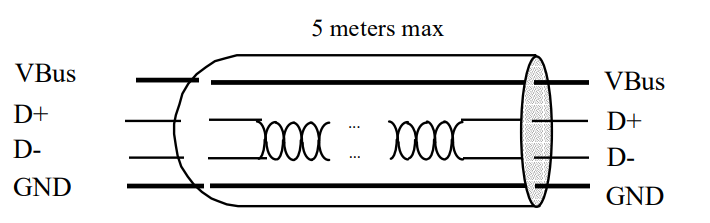
\includegraphics[width=0.5\linewidth]{usbsingalgraphic.png}
    \caption{USB Cable Signals}
    \label{fig:usbsingalgraphic}
    \cite{WaybackMachine2018}
\end{figure}

In figure \ref{fig:usbsingalgraphic} we can see how a USB cable is constructed. \\
The connection is built upon four signal lines; a negative (Ground) powerline GND, a positive powerline VBUS for the power supply, and two data transfer lines D+ and D-. The two physical transfer data lines are aligned as a twisted pair. This alignment protects them from outside electrical noise and does not mean that more than one logical line is available. They work together to transmit one logical signal, one single bit. USB utilizes Non Return to Zero Inverted (NRZI) meaning that the bits on the bus are represented by a transition of physical levels, rather than the presence or absence of them. A powerchange during a time interval signals a 1, if the connection stays constant, it's a 0. This allows data transfer while simultaneously allowing the participating parties to synchronise their bit clocks.  \\
Since there is only one logical data line, data transfer can only happen in one direction at a time. Bi-directional communication happens in half-duplex mode; the parties alternate. To deal with this restriction, a protocol that manages data and sender order has to be followed; the USB protocol.  

This next section will expand on the functionalities of the USB protocol as described by \cite{nissimUSBbasedAttacks2017}. 

A USB connection includes a host, usually a computer, and one to many peripheral devices that connect to the PC's embedded USB hub.  \\
USB devices generally fit into two categories; I/O devices that add capabilities to the host, and hub devices which connect additional devices to the host. An USB cable has two main functionalities; Establishing a data connection to allow communication between the connected parties, and supplying electrical power to the connected peripheral device if it is not self-powered. Such devices that draw power from an USB Host are called bus-powered. \\ 
For bus-powered devices it is important to receive the power from the UBS cable before it is supposed to process any data, which is why the USB connector was specifically designed with power pins that are longer than the signal pins.\\
Every USB device is equipped with a microcontroller chip that manages the USB interactions with the host, and optionally also has a bootloader that allows loading firmware, for example for updates. \\
One USB device consists of one to multiple logical subdevices that are known as device functions. For a webcam with built in audio this would correspond to a video and an audio function. Devices with multiple subdevices are referred to as composite devices. Each functions is managed through a separate endpoint on the bus with it's own logical address. One endpoint forms a logical communication channel called a pipe, of which there are two types.  
\begin{enumerate}
    \item Message Pipe: A message pipe is used for control transfers. That means they are used for short and simple commands sent to the USB device and status responses to the host.
    \item Stream Pipe: A stream pipe is used for actual data transfer.
\end{enumerate}
Data transfer can only take place if the host directly requests it. An USB device cannot transfer information autonomously. 

In order to be able to communicate with any USB device, a connection needs to be established and initialized. This is done with a process called 'enumeration' that starts as soon as the physical connection is established. It consists of four main steps;

\begin{enumerate}
    \item \emph{Detection}: A change in the current on the data lines is detected by the host, so it knows that a new USB device has been connected.
    \item \emph{Device Speed}: The speed of the device is determined by using the change on  the data lines in step 1.
    \item \emph{Device Descriptors}: The USB device is reset by the host through a specific dataline signal. This prompts the device to send information about itself (it's descriptors) to the host by which it is identified.  \\
    The exchange of descriptors follows a defined order; 
    \begin{itemize}
        \item First the host will request the descriptor length and the descriptor from the device with the Get\_Device\_Descriptor command.
        \item The advice is reset again and given a unique local address by the host called via the Set\_Address command. 
        \item Lastly, the device is prompted to send it's configuration by the Get\_Configuration\_Descriptor. The configuration includes a hierarchy of interface, endpoint and class specific descriptors.  
    \end{itemize}
    \item \emph{Loading Drivers}: Now that all the information has been exchanged the host can start using it to load the device specific driver's that will allow it to be controlled. The corresponding driver is found by the USB class, the vendor ID (VID) and the product ID (PID). Most standard drivers are included in the OS of the host, if they aren't the user has to download them manually. This concludes the enumeration process, after these steps the device is ready for use.
\end{enumerate}




\section{The Dangers of USB} \label{TheDangersOfUSB}

Some people might notice that during the initialization process described in section \ref{TheUSBProtocol} there are no verification or authorization steps. The protocol assumes that any physically connected USB device is trustworthy and does not take any precautions to check its claims and properties. \\
This is a big oversight and opens the door for a lot of malicious activity. 
The risks posed by this activity is exacerbated by the fact that USB devices are not perceived as a threat by a vast majority of people. In fact, many would absolutely pick up, plug in, and even interact with USB sticks they find lying around on the ground. A study \cite{tischerUsersReallyPlug2016} conducted in 2016 found that USB sticks are a very effective attack vector. They explored whether USB sticks dropped on a university campus would really be picked up and plugged in. They found that users opened one or more files on 45\% of the flash drive and that 98\% of the drives were removed from the drop location by the time the experiment had ended. Based on this, the authors estimate that between 45\% and 98\% of drives were eventually plugged in. On the drives the authors placed information for a survey to explore the finder's motivation. From this survey it was concluded that the USB drives were plugged in mostly out of altruistic motives (to find the owner). The social engineering attack was an "expeditious" vector with a median time of connection of only 6.9 hours.  \\
USB ports are common also in public, for convenient charging on the go, for example in Buses or Airports \cite{kumarJuiceJackingUSB2020}. People rarely think twice when they connect their laptop to an external display in a library or accept a charging cable from a friend. None of these actions are protected, and every interaction through the USB protocol poses a risk most are not aware of.

A myriad of different attacks are possible through such an unsecured attack vector.\\
Through USB, data can be silently downloaded without the user's permission or knowledge from computers \cite{clarkHardwareTrojanHorse2009} as well as phones \cite{SharpIdeasDownloads2006}. USB drives developed to be able to do data manipulation, and with the increased popularity of U3, attackers could hack U3 images and replace them for their own malicious purposes to take advantage of auto-run. 
How much damage could be done with this is best exemplified with Stuxnet \cite{kushnerRealStoryStuxnet2013}. It's a malware program that could travel via USB; a computer that came in contact with an infected USB stick would immediately be compromised. In this way, malware could spread even in an air-gaped environment. The highly sophisticated and targeted attack was discovered in 2010 and is confirmed to have damaged centrifuges that were part of Iran's Nuclear Program.\\
But an attack via USB does not have to have the dimensions of an (alleged) geopolitical intelligence mission \cite{kushnerRealStoryStuxnet2013}, there are more examples of day-to-day threats to exemplify what USB can do. On Windows XP it is possible to emulate a CD-ROM device through an USB connection and hack the U3 autoplay feature \cite{al-zarouniRealityRisksConsented2006}, data can be exfiltrate from iOS6 through a USB charging cable \cite{lauMactansInjectingMalware2013}, USB can be used to propagate attacks from one computer to another, as demonstrated in \cite{wangExploitingSmartphoneUSB2010}, or destroy a target with power surges that irreparably damage the host \cite{USBKillDevices}, Fork Bomb attacks can be launched via USB \cite{efendyExploringPossibilityUSB2019}, and, most importantly, since USB does not require authentication, it can be used to emulate other devices, namely devices that are used for human input. Human Interface Devices (HID) such as keyboards and mice present an unparalleled attack vector, where a hacker with physical access to an unlocked computer can remotely execute any action a user themselves could \cite{USBRubberDucky}, \cite{MGCable2019a}, \cite{lawalFacilitatingCyberenabledFraud2022}. \\
How such HID attacks could look like, and the extent their damage can reach, will be discussed and exemplified in section \ref{Methodology}.

\subsection{Bad Hardware}

None of the attacks and only part of the defenses that are discussed in this thesis would be possible without specialized hardware. This section will therefore give a brief introduction into the different microcontrollers and computers that will be mentioned in the following chapters.\\
In general, any USB deivce that has been modified to execute some malicious action will be referred to as BadUSB, a term coined by a BalckHat presentation by Karsten Nohl, Sascha Krissler, and Jakob Lell \cite{Srlabsbadusbblackhatv1Pdf2014}. 


\subsubsection{Arduino}

\begin{figure}[H]
    \centering
    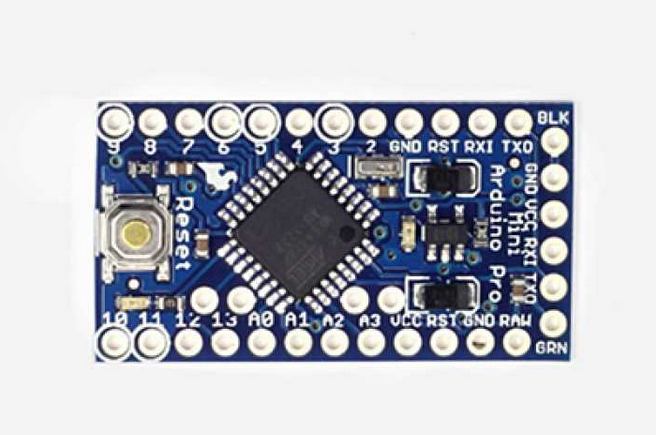
\includegraphics[width=0.25\linewidth]{arduinomini.png}
    \caption{The Arduino pro mini, used by \cite{bojovicRisingThreatHardware2019}}
    \label{fig:ArduinoProMini}
    \cite{ArduinoProMini}
\end{figure}
Arduino \cite{ArduinoHardware} is a company that produces a range of different small microcontrollers designed to be accessible and straight forward. They are supported by the open-source Arduino platform and the Arduino IDE \cite{ArduinoArduino2024}.


\subsubsection{Teensy}

\begin{figure}[H]
    \centering
    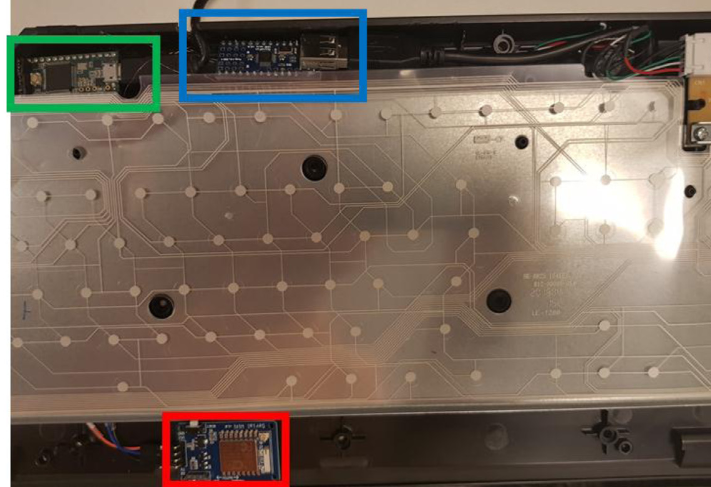
\includegraphics[width=0.5\linewidth]{teensy.png}
    \caption{Teensy (in green) as built into Malboard}
    \label{fig:builtInTeensy}
    \cite{farhiMalboardNovelUser2019}
\end{figure}

The Teensy  \cite{TeensyUSBDevelopment} is a microcontroller system based on USB, that is, as it's name suggests, tiny. It can be programmed via it's USB port, is compatible with Arduino Software and works with Mac OS, Linux, and Windows. It comes standard with solder pads. To program it, the Teensy Loader Application can be used.
A teensy can be programmed to emulate a keyboard and a mouse and change its PID and VID \cite{farhiMalboardNovelUser2019}.\\
These qualities, especially it's size, make it a popular microcontroller for self made BadUSBs. 


\subsubsection{Hak5 Hardware} \label{Hak5Hardware}

\begin{figure}[H]
    \centering
    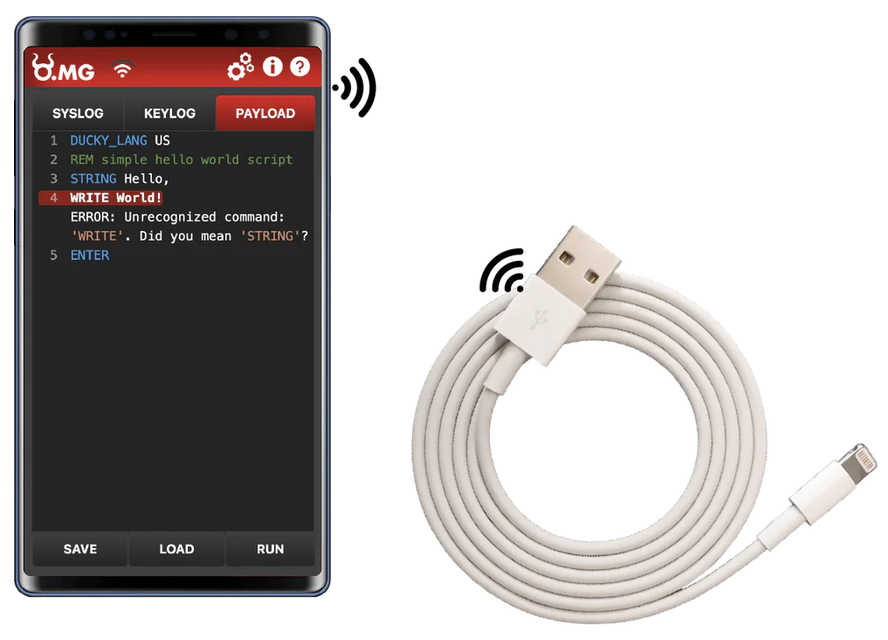
\includegraphics[width=0.5\linewidth]{OMGCable.png}
    \caption{The O.MG cable and it's Web IDE open on a phone}
    \label{fig:OMGCable}
    \cite{hak5MGCable}
\end{figure}

Hak5 is a company founded in 2005 by who have made it their missions to 'advance the InfoSec industry' \cite{hak5}. They have an award winning podcast, a big YouTube channel, and a lot of penetration testing gear. They aim to inform people of the security risks that come with tech with the goal of ultimately making the world a safer place. \\
In 2019, the O.MG cable was made available at Hak5 \cite{MGCable2019a} marking the beginning of a collaboration between the creator of the O.MG cable and founder of Mischief Gadgets, MG \footnote{https://twitter.com/_MG_} and the Hak5 team. They have since released many variations of the O.MG cable, including a plug, an adapter, an 'unblocker', and a cable detector \cite{hak5MischiefGadgets}. The device that will be featured in this thesis is the O.MG cable. It is essentially plug and play and can therefore be used to conduct injection attacks, without having to do any hardware building yourself \cite{hak5MGCable}. 



\section{DuckyScript and the O.MG cable}


This section will give an overview over the O.MG cable, and the scripting language it is equipped with; DuckyScript. 

\subsection{The O.MG cable} \label{theOMGCable}

As described shortly in sections \ref{Hak5Hardware} and \ref{HistoryOfAttacks} the O.MG cable is a BadUSB cable invented by MG \cite{MGCable2019a}, produced by Mischief Gadgets \cite{hak5MischiefGadgets} and sold in cooperation with Hak5 on their website \cite{hak5MischiefGadgets}. \\
The cable does not have any physical markers; neither it's USB ends, the cable, nor the weight gives any indication that it has so many more capabilities than other USB cables. For the most part, it is a usual USB cable; the non-active (passthrough) end does not have any special abilities, and if it is not configured to execute a boot script, the cable can be used like any other to charge an transfer data. It's malicious active end is marked by a USB trident as found often on USB cables to indicate their compatibility with the USB standard. That end transmits the payloads on the device to the USB host. It is available in USB-A, USB-C and lightning. 
When setting up to use a O.MG cable ,the very first thing that has to be done is flashing it. The cable has to be flashed before it is used, or after a self-destruct was triggered. To flash it, a O.MG Programmer is needed \cite{hak5MGCable}. The active end of the O.MG cable is plugged into the programmer, which itself is connected to a computer by a regular USB data cable. Flashing can either be done with the official open source firmware \cite{DuckyScriptSyntaxGuide} via the website \footnote{https://o.mg.lol/setup/OMGCable/} or with custom firmware. \\  
Once the device has been flashed, it is ready to be used. Once an active end received power from a USB host, it established a small Wifi network, with the default SSID O.MG and password 12345678, both of which can be changed. Through that network the WebUI to control the cable can be accessed via http://192.168.4.1 . \\
The WebUI offers a lot of different features [TODO; add screenshot of the webUI]

\begin{enumerate}
    \item Payloads
    \item Geofencing
    \item Self-Destruct
    \item Keymap Viewer
    \item Keylogger
    \item Partition Editor
    \item C2
    \item HIDX StealthLink
\end{enumerate}

The following subsections contain a short description of each of these features. 

\subsubsection{Payloads}

All O.MG devices that can be programmed for keyboard injection support an enhanced version of DuckyScript. Basic Duckyscript, as expanded upon in section \ref{DuckyScript} does not support all the extra features of the O.MG devices, such as self-destruct of GeoFencing. \\
Payloads can be written directly in the WebUI, where they can be stored into slots. Depending on the model, the cable supports from 8-200 payload slots \cite{hak5MGCable}. They can be directly executed in the WebUI (executed on the host connected to the active end), simply stored, modified, and accessed, or set as a bootscript. Only one payload can be a bootscript; it is the script that is executed as soon as the active end is connected. \\
USB overlock is a feature only available on the elite model that allows sending HIDX packets about 8 times as fast as usual. This can mean that the data is sent faster, than the host can receive it, in which case it is lost. 


\subsubsection{Geofencing}

Geofencing can be accomplished by a simple conditional statement. It can trigger or block actions depending on the presence or absence of a wifi network with a specific SSID. This is accomplished by a condition that is evaluated every time the O.MG device powers up. Alternatively, the cable can wait until a SSID or BSSID is present with the 'WAIT\_FOR\_PRESENT' keyword. It will either wait for a specific amount of time or run forever. Completing this feature, it is also possible to wait until out of reach of a network.  

\subsubsection{Self-Destruct}

Cleanup is an important part of an attack or pentetration test. This cable supports two kinds of self-destruct that can be triggered via the WebUI or with a keyword in the code.
\begin{itemize}
    \item  \textbf{Self-Destruct 1:} Completely erases all data on the cable and disconnects the data line. The cable will appear broken. To use it again, it has to be physically recovered and reflashed.  
    \item  \textbf{Self-Destruct 2:}  Erases all the data but retains the data lines, turning the cable in a normal USB cable. Reflashing is also necessary to use the cable again. 
\end{itemize}


\subsubsection{Keymap Viewer}

Since the O.MG cable imitates keyboard presses, it is dependent on the keyboard settings of the attacked host. Input in a US keyboard will not produce the same signal to the computer as a DE\_CH keyboard even though the same key is pressed. For this reason, the lanugage of a payload has to be set, which is explained in more detail in section (TODO!!). If the keyboard settings of the target are not known beforehand, obtaining this information in the reconnaissance phase is crucial. \\
For this reason the Keymap Viewer exists. Through the WebUI the keyboard layout of a connected host can be determined. (TODO; try this out!!)

\subsubsection{Keylogger}

When an O.MG cable is connecting a physical keyboard with a detachable cable to a host, it can keylog the strokes from the keyboard and display them in real time on the WebUI. In order for this to work, the keyboard has to be Full Speed USB (12mbps) and not low (1.5mbps) or high speed (480mbps) 

\subsubsection{Partition Editor}

On specific models of the O.MG cable a user can device themselves how the available storage should be used with the partition editor. They can decide to redirect storage resources to payload slots, individual slot size, size of storage for exfiltrated data, or keylogging storage. 

\subsubsection{C2}
A C2 server eliminates the need for physical proximity to the O.MG device to connect to and communicate with it. The cable can connect to the C2 server as well as the attacker. This way it can be controlled from anywhere. 

\subsubsection{HIDX Stealth Link}
This feature is still in progress, but the idea is to enable more stealthy data exfiltration. Instead of establishing a network or sending the data via the host, the cable relays the data via the HID channels.  


\subsection{Ducky Script} \label{DuckyScript}

DuckyScript was invented by Darren Kitchen, the founder of Hak5. It evolved from a macro scripting language that could handle keyboard injections and delays in it's first iteration to a structured and feature rich programming language supporting injection attack specific commands (jitter, side-channel exfiltration) as well as control flow instructions, repetitions and functions in version 3.0. \cite{the book} [TODO cite the book!!] \\
Some specific Hak5 gear like the BashBunny or LANTurtle use an interpreted version of DuckyScript 1.0 that couples the BASH shell scripting language. \cite{Hak5Usbrubberduckypayloads2024} The DuckyScript version licenced for the O.MG cable is based on DuckyScript 1.0 and additionally includes some device specific commands for the specific functionalities of the O.MG cable. The available DuckyScript 1.0 commads are limited to REM (marks a comment), DELAY (pauses the payload), STRING (injects keystrokes) and some buttons like ENTER, GUI, F11, PAGEUP, TAB; ESCAPE etc. \\
A basic implementation of a Hello, World! Program for the O.MG cable could look like this:

\begin{verbatim}
REM Title: Hello, World!
REM Description: Write Hello, World! in the terminal
REM Target: Windows (including Powershell 2.0 or above)

DELAY 3000
GUI r
DELAY 750
STRING cmd
ENTER
DELAY 2000
STRING Hello, World!
\end{verbatim}



\section{Chapter Conclusion}

This chapter introduced the USB standard and protocol and the vulnerabilities that come with it. \\
It explained, how the lack of USB authentication can be leveraged by malicious actors to target users, in a stealthy and efficient way. 
Lastly, a basic overview over the hardware in this thesis was given and the O.MG cable, as well as it's scripting language, DuckyScript was introduced. 
\chapter{Related Work}

\section{Introduction}

Since the release of USB in 1996 \cite{WaybackMachine2018} black (malicious) and white (benevolent) hats (hackers) have equally pursued the development of increasingly sophisticated methods to attack and defend, respectively. This chapter will expand on their works chronologically and thereby illustrate the lengths both sides have gone to fight for the upper hand in this co-evolution.\\
However, it has to be kept in mind that even the most sophisticated defense techniques have weaknesses, the biggest of which is the user itself. Social Engineering attacks are infamous, and can be infamously effective \cite{krombholzAdvancedSocialEngineering2015}. Unless it is physically impossible to attack a USB device to a host, there will always be a way to convince an unsuspecting target to plug it in for you.\\ 
Similarly, HID attacks can fail for the most mundane reasons. This form of attack is not very flexible, and an unexpected pop-up, a keystroke by the user at the wrong moment, or one small timing miscalculation could fatally influence the attack. This problem will be expanded upon in section !!TODO!!\ref{}.\\
Nevertheless, the risk of a hack makes it worth for both sides to put in the effort, as documented in the following subsections.

\section{Attack}

To get an overview over the different types of attacks that are possible with USB one can refer to Nissim et al. (2017) \cite{nissimUSBbasedAttacks2017}. In their paper they classified 29 different USB based attacks into 3 main categories and 2 subcategories. They distinguish the attacks by the Hardware that was used. The categories are: Programmable Microcontrollers, Electrical, and USB Peripherals. The last one is further split into USB maliciously re-programmed peripherals and non re-programmed peripherals. 

\begin{enumerate}
  \item Electrical USB based attacks: Most notably the USB Killer attacks; a device that can discharge high voltage power surges with the goal of damaging the device it is plugged into. \cite{USBKillDevices}
  \item Programmable Microscontrollers: Rubber Ducky, USBdriveby, Turnipschool, URFUKED.
  \item Peripherals:
  \begin{itemize}
      \item Re Programmed Peripherals: smartphone based HID attacks, iSeeYou attack
      \item Non-Reprogrammed Peripherals: USBee attack, Stuxnet
  \end{itemize}
\end{enumerate}
	


This thesis will focus on the category programmable microcontrollers. In the following section we will see a chronological overview over how the programmable Microcontrollers have evolved.  

\subsection{History of Attacks} \label{HistoryOfAttacks}

One of the first documented attacks conducted via USB, was done using a tool called Slurp \cite{SharpIdeasDownloads2006} which was available as early as 2006 and could attack an IPod via a charging cable to search through it's files looking for certain file extensions. While in theory it was claimed that the implementation could be modified to extract the files that it has found, this implementation only displays the number of matching files that were discovered, since it was meant to raise awareness and not to be used for malicious purposes. 

In the same year \cite{al-zarouniRealityRisksConsented2006} published a paper demonstrating another early version of the USB attack utilizing a functionality called U3, which was developed to allow users to carry portable applications on USB sticks. The USB stick in question would pose as two pieces of hardware; a CD-ROM device and a USB storage device. The attack can then be mounted by hacking the auto-run feature of CD-ROM. This meant, code could be executed automatically on the target machine only via the USB stick. 

In 2009 \cite{clarkHardwareTrojanHorse2009} described an data exfiltration process via USB that they called a Hardware Trojan Horse. This Trojan was built into a keyboard for disguise and used it's "unintended" USB channels; the keyboard LED and audio channel function as a communication tool from the computer to the keyboard and could therefore be repurposed to exfiltrate data. This network endpoint data could then be searched for sensitive information and the findings be sent to the attacker. With their paper the researchers wanted to raise awareness for this kind of attack, they write; "Physical access can now be potentially sufficient to compromise a network endpoint, without attempting access through the network." \cite[p.~7]{clarkHardwareTrojanHorse2009}.
Expanding on their work with data exfiltration, Clark et al.\cite{clarkRisksAssociatedUSB2011} released a paper in 2011 demonstrating how peripheral hardware Trojans can be used to execute code on the USB host \cite{clarkRisksAssociatedUSB2011}. 

2010, Wang and Stavrou \cite{wangExploitingSmartphoneUSB2010} were the first to describe attacks propagated via USB while launched from a smartphone or computer. They demonstrated propagation from Phone to Phone, Phone to Computer and Compute to Phone.

At Defcon 2010 Adrian Crenshaw presented an USB dongle he called Programmable HID USB Keystroke Dongle (PHUKED) and later published the instructions on how to build it on his website \cite{ProgrammableHIDUSB}. The penetration testing device was built using a Teensy microcontroller. It could be programmed to spoof a keyboard and emulate keystrokes on an unlocked computer. 

The company Hak5 launched the first version USB Rubber Ducky in 2010 \cite{USBRubberDucky}. It is a commercially available, closed source keystroke injection tool disguised as a normal USB flash drive. It runs on it's own scripting language called DuckyScript, that has seen 3 versions already, with the newest one even supporting control flow constructs, repetitions, and functions. The Rubber Ducky has a UBS A and a USB C end \cite{USBRubberDucky2023}. This step into commercialisation made the USB attack widely accessible. You don't have to be a proficient hobbyist to make a BadUSB yourself, instead you could just buy one for 80 USD\cite{USBRubberDucky2023}. Furthermore, since Hak5 has a big comunity, this raised a lot of awareness for the existence of this attack vector. 

Lau et al., 2013 \cite{lauMactansInjectingMalware2013} showed that attacks on iOS6 using USB are possible. Within one minute of being plugged into the charger cable, the phone was compromised. The approach leverages USB to bypass Apple's security mechanism protecting their devices from arbitrary software installation. On top of the malware installation, the malware can be hidden from the user in the same way as Apple hides their own built-in-applications. The hardware the authors designed for this study is called Mactans and uses a BeagleBoard.
With iOS 7 Apple already implemented the protective measures proposed by this paper an thereby patched this particular attack vector. 

While all of these developments were impressive and pushed the field forward, it is not known when exactly government actors joined the field of research around USB attacks. However, in 2013 a story by the German newspaper Der Spiegel revealed that the US government had been conducting significant research in this area \cite{appelbaumCatalogRevealsNSA2013}. Developed by the NSA, one of the first USB based man-in-the-middle attack tools, Cottonmouth could be built into keyboards or accessory cables. It is part of a large collection of tools developed for the NSA called the ANT-Catalogue \cite{InteractiveGraphicNSA}. In the device catalogue Cottonmouth is advertised as a "hardware implant which will provide a wireless bridge into a target network as well a the ability to load exploit software onto target PCs". This very early attack tool was was only available in batches of 50 for a total price of 1'015'000\$ (20'000\$ / piece).

The NSA playset project is an open source project that tries to replicate the technologies revealed in the ANT-Catalogue \cite{NSAPlaysetTurnipschoolHtml}. Michael Ossman replicated Cottonmouth as a part of this  project with a device called Turnipschool, making the technology available to the public. \footnote{A full instruction on how to build it can be found on the GitHub page of the NSA-Playset Project \cite{NSAPlaysetTurnipschoolHtml}.}

USBdriveby was developed by Samy Kamkar in 2014 \cite{SamyKamkarUSBdriveby}. USBdriveby is a device that can simulate keyboard and mouse input to install a backdoor and override DNS settings in order to control the flow of network traffic within seconds of being plugged in via an USB on a Windows machine. The device is built on a teensy microcontroller and can be worn as a necklace.

In August of 2014 Karsten Nohl, Sasch Krissler, and Jakob Lell presented their research on USB attacks at the BlackHat Convention \cite{Srlabsbadusbblackhatv1Pdf2014}. They had reverse engineered and patched USB firmware in such a way that they created a useable, programmable, well disguised USB attack tool form a normal USB flash drive. They called it Bad USB. It could emulate Keyboard input and even spoof an Ethernet connection, allowing a connected device to intercept all internet traffic from the attacked computer. Furthermore the device can be used to mount a boot-sector virus, prompting a computer to boot an operating system from the stick, or if necessary, emulate the keystrokes to initiate the boot from the USB stick.f This presentation reached a big audience and caused a stir, inspiring many subsequent papers.

Han et al.\cite{hanIRONHIDCreateYour2016} developed a framework called IRON-HID in 2016 that can be used for penetration testing. It attaches to the existing USB devices turning them into Bad USBs. The hardware attachment can built either with Arduino or Teensy. On top of that they constructed a framework to use the hardware for various penetration testing scenarios like brute force keyboard injections to guess PIN codes of smartphones or to test whether CD-ROM programs are automatically executed. Also part of the framework are a test agent program, and a commander program, giving the penetration tester ways to reliably execute and monitor their tests.   

Video Jacking is an attack demonstrated by Brain Kebs \cite{RoadWarriorsBeware2016} at Defcon 2016. He built a demonstration to raise awareness for USB based attacks by putting up a booth that would 'charge' your phone. Once the phone was connected, however, the video feed from the camera was shown on a monitor without any additional action by the user. 

Inspired by PHUKED, \cite{elkinsHackingHardwareIntroducing} released an improved version of the USB Dongle at Defcon 2018, called URFUKED based on Arduino that can additionally mount an HID attack by triggering it remotely.  

Another proof of concept was published by \cite{bojovicRisingThreatHardware2019} in 2019. In their paper they documented how they implemented a keystroke logger and bad USB in the keyboard of one of their colleagues using an Arduino microcontroller. They recorded the target's keystrokes on a built in SD card that they then retrieved. The data was analyzed to sensitive data such as login information. In the next step they used their findings to contrive a custom script to exploit the Virtual Network Computing (VNC) service the target was using to gain remote control overt the target machine. 

\label{malboard}2019 saw the developement of a novel attack called Malboard \cite{farhiMalboardNovelUser2019}; Previously, detection of a keyboard attack was easy by identifying the keystroke dynamics as artificial (as discussed in section \ref{HistoryOfDefense}). Malboard instead generates keystrokes that pass for the attacked user's and thereby bypass the simple detection mechanism. In order to achieve this, the user's keystrokes are observed, analyzed and emulated. To predict keystroke dynamics that may not be present in the keylogging data, a technique based on a clustering method is used. Two types of attacks can be executed with Malboard: 
\begin{enumerate}
    \item By combining the modified keyboard with either Remote Server Injection (RSI), where keystroke logs are either analyzed locally or sent to the off-site server to create the user profile. In a second step that off-site server sends the malicious payload using a cellular or Wifi connection. 
    \item Alternatively Malboard is used with Physical Access Injection (PAI) where the profile is made locally through Malboard and once the attacker has gained physical access to the keyboard, their malicious keystrokes will be sent to the computer in the timing on the actual user's profile. 
 \end{enumerate}
 Malboard was able to evade existing detection mechanisms in 83\% - 100\% of cases. It was able to fool DuckHunt everytime, while evading detection by Typing DNA and KeyTrac, two private keystroke authentication programs, in 83-93\% of cases. The researchers also proposed ways to defend against their attack, which will be discussed further in the detection section \ref{HistoryOfDefense}. \\
 This attack technique is a game changer because it can evade the first level of defenses that focus on typing patterns and speed, which is the most intuitive way of blocking an HID injection attack. While that means that it might trick many systems that are put in place by a target, it also eliminates one of it's biggest strength; speed. Typing at a normal speed gives the user time to notice and interrupt the attack.  


Efendy et al. 2019 \cite{efendyExploringPossibilityUSB2019} showed that a fork bomb attack on Windows 8 can be carried out via USB. Fork Bomb is a Denial of Service (DoS) attack that creates new processes repeatedly thereby depleting system resources. The computer will run out of memory, causing errors. The user will no longer be able to give any input to the computer. Ultimately it will exhaust the resources of the OS, overtaxing the kernel causing a crash.  

The O.MG cable is a handmade cable that poses as a normal USB cable with data transfer and charging capabilities \cite{hak5MGCable}. However, inside, there is an implant that can mount sophisticated HID spoofing attacks. It was first released in 2019 with prototypes available at Defcon \cite{MGCable2019a}, is now commercially available on the Hak5 Website. It supports KeyStroke injection via DuckyScript, mouse injection, has 8-200 payload slots (depending on the version), a deployment speed of 120 - 890 keys/sec, a self destruct feature, supports geo fencing, 192 different keyboard layouts, and wifi triggers. The elite version also has a hardware keylogger, supports HIDX Stealth link to set up remote servers, and extended WiFi range and stealth optimized power draw. 
You can choose between a USB A or C, mini USB, and lightning ends. To use them you have to activate them and upgrade to the latest firmware with the programmer. \\
This attack vector is especially vicious because while many people have been made weary of USB sticks by this time, no one thinks twice about plugging in a charging cable, after all, it is only a cable, it's sole purpose is to transmit electricity, right?

In 2020 Dr. Kumar described a type of attack possible via USB called 'Juice Jacking' \cite{kumarJuiceJackingUSB2020}. It is a type of attack that specifically involves a malicious charging port (possibly in public) that initiates an attack when a device is connected, either installing malware or copying sensitive data from the device. He explains that this is possible, because the data transfer mode on phones is enabled by default. 

In the same year, Muslim et al. \cite{muslimImplementationAnalysisUSB2020}, implemented a demonstration of how a USB attack can be leveraged to steal passwords stored in the browser of a Windows 10 PC using the Arduino Pro Micro Leonardo.  They proved that it is possible to use keyboard injection to download scripts from GitHub to extract stored passwords from Chrome and Firefox and then send them to the email address of the attacker. 

Lawal et al. \cite{lawalFacilitatingCyberenabledFraud2022} 2022 were the first ones to publish a paper in which they used an O.MG cable to execute USB attacks. In their work they showed that it is possible to carry out an attack through which a document is edited in such a way that it is impossible to tell whether the modifications were made by the cable or the user of the machine. The device seems to be "capable of perfectly modifying records and files without the forensic tools being able to differentiate between files modified by the user and files modified by the O.MG Cable". Although it is possible to find hints of the presence of an O.MG cable, it cannot be determined which actions were carried out by the cable and not by the user. The authors stress, that this can be misused to place incriminating information or otherwise alter the state of information on a PC in a harmful way, while framing the user of the machine. 


\Rotatebox{90}{%
\begin{tabular}{|c c c c c c|} 
 \hline
 Name & Author / Inventor & Year & Charcteristics & Hardware & Software \\ [0.5ex] 
 \hline \hline
 pod slurping & Sharp Tools \cite{SharpIdeasDownloads2006} & 2006 & iOS slurping via Lightning Cable &  &  $\times$ \\
 \hline
 -  &  Al-Zarouni \cite{al-zarouniRealityRisksConsented2006} & 2006 & stick / CD-ROM & & $\times$\\
 \hline
 Hardware Trojan & Clark \cite{clarkHardwareTrojanHorse2009} & 2009 and 2011 & built in keyboard and audio & $\times$ & $\times$ \\
 \hline
 - & Wand and Stavrou \cite{wangExploitingSmartphoneUSB2010} & 2010 & attack propagated by USB & & $\times$\\
 \hline
 PHUKED & IronGeek  (Adrian Crenshaw) \cite{ProgrammableHIDUSB} & 2010 & stick / 'dongle' & $\times$ & $\times$  \\
 \hline
 USB Rubber Ducky & Hak5 \cite{USBRubberDucky} & 2010 & Stick & $\times$ & $\times$ \\
 \hline
 Mactans & Lau et al. \cite{lauMactansInjectingMalware2013} & 2013 & IOS6 attack & $\times$ & $\times$ \\
 \hline
 Cottonmouth & NSA \cite{appelbaumCatalogRevealsNSA2013} & 2013 & cable / built-in & $\times$ & $\times$ \\ 
 \hline
 Turnipschool & NSA-playset \cite{NSAPlaysetTurnipschoolHtml} & 2015 & cable / built-in & $\times$ & $\times$ \\
 \hline
 USB Driveby & Samy Kamkar \cite{SamyKamkarUSBdriveby} & 2014 & USB 'stick' & $\times$ & $\times$ \\
 \hline
 Bad USB & Nohl et al.\cite{Srlabsbadusbblackhatv1Pdf2014} & 2014 & programmable HID spoofing USB Stick & $\times$ & $\times$\\
 \hline
 IRON-HID & Han et al \cite{hanIRONHIDCreateYour2016} & 2016 & DIY Framework & $\times$ & $\times$ \\
 \hline
 - & Brian Kebs\cite{RoadWarriorsBeware2016} & 2016 & Video Jacking & & $\times$\\
 \hline
 URFUKED & Monta Elkins \cite{elkinsHackingHardwareIntroducing} & 2018 & USB stick & $\times$ & $\times$\\
 \hline
 -  & Bojovic \cite{bojovicRisingThreatHardware2019} & 2019 & built-into keyboard & $\times$ & $\times$ \\
 \hline
 Malboard & Fahri et al. \cite{farhiMalboardNovelUser2019} & 2019 & keystroke profiling & $\times$ & $\times$\\
 \hline
  - & Efendy\cite{efendyExploringPossibilityUSB2019} & 2019 & Fork Bomb Attack & & $\times$ \\
 \hline
 O.MG Cable & MG and Hak5  \cite{hak5MGCable} \cite{MGCable2019a} & 2019 & USB Cable & $\times$ & $\times$ \\
 \hline
- & Kumar \cite{kumarJuiceJackingUSB2020} & 2020 & Juice Jacking & $\times$ & $\times$ \\
\hline
- & Muslim \cite{muslimImplementationAnalysisUSB2020} & 2020 & stealing passwords & & $\times$ \\
\hline
-  & lawal \cite{lawalFacilitatingCyberenabledFraud2022} & 2022 & O.MG cable attack & & $\times$ \\
 \hline 
\end{tabular}
}%

\section{Defense} \label{HistoryOfDefense}

The previous section outlined the evolution of attack tools, this sub-chapter will contrast that with the evolution of counter measurements. 
The following section is partitioned into two categories; active prevention and passive techniques focused on attack detection.

\subsection{Active Defense}

One of the first published defense systems was USBGuard \cite{HomeUSBGuard}, released in 2014. It is a Linux-based Daemon that implements black- and whitelisting of USB devices based on user defined rules. To this end, it supports it's own specific rule syntax \cite{RuleLanguageUSBGuard}. The devices are identified through their name, serial number, port, and interface type. These values are then stored in a hash. The custom rules furthermore support time based attributes and random values. This system is only available on Linux and has been accused of being unsafe by \cite{farhiMalboardNovelUser2019} since the device identification metrics be be spoofed by a Teensy. 

GoodUSB \cite{tianDefendingMaliciousUSB2015} is a program that relies on user input to defend against malicious USB. It features a graphical interface that prompts users to select the device class they expect and then compares that expectation with the information given by the device itself. If the two don't match, access to the computer is denied. After an initial registration of the devices by the user, the program will not ask for verification again on future contact. This way, when the user plugs in a BadUSB, the device will register as USB storage stick and GoodUSB will only allow actions compliant with the behaviour of an USB stick. Any HID spoofing will be blocked.
\cite{nissimUSBbasedAttacks2017} criticizes that GoodUSB assumes all devices are in an uncompromised state when first contact is made. It is not guaranteed to work with infected hosts (for example Teensy built into a keyboard). 
\cite{mohammadmoradiMakingWhitelistingBasedDefense2018} criticizes this approach as missing a reliable solution for uniquely identifying registered USB devices. In cases of the devices using base class code, spoofing would still be possible, the same is true for devices using vendor specific interfaces (mostly cellphones). 

The Idea of Cinch \cite{angelDefendingMaliciousPeripherals2016}, a defense mechanism developed in 2016, is to treat peripheral devices, like USB devices on a kernel level as though they were untrustworthy network endpoints. To this end it would build an extra layer between the device and the computer, channeling traffic through a 'choke point' where the actual defense would take place. These defenses, called 'policies' in the context of Cinch, include static rules (pattern matching) or checking specifications of expected devices against actual traffic. 
These modifications do not require changes to the computer hardware, nor do they impose an unreasonable overhead to the system.
\cite{farhiMalboardNovelUser2019} describes Cinch as "Middleware that behaves as a separation layer between the host computer and the USB device." However, they critique: "USB attacks can be mutated and randomized to avoid detection by those kinds of mechanisms." \cite[p.~7]{farhiMalboardNovelUser2019}

SandUSB (2016) consists of a physical middleware and user interface to control and monitor USB devices connected to a host \cite{loeSandUSBInstallationfreeSandbox2016}. Furthermore it features automatic defensive measures, five of which come out of the box: blacklisting, keyboard dynamic analysis, files and settings modification detection, input pattern matching and USB packet analysis. Further semi automatic measures can be configured through the UI. 
During enumeration, USB device information such as PID, VID and device class are presented to the user. A user can spot a spoofing device by the displayed device class and blacklist the device immediately if they wish.
Additionally the keyboard dynamics analysis detects malicious input by unusual speed and typing patterns. Should a USB device try to access sensitive settings and files, SandUSB can block the access to prevent attacks. Lastly, the authors claim to detect malicious payloads, although they do not specify how. 

USG \cite{robertfiskRobertfiskUSG2016} is a hardware USB firewall designed in new Zealand. It was design to prevent supply-chain attacks, and has an open source firmware that can even be custom written. It limits the speed of packets o 12Mbps, protecting against high speed injection attacks. Furthermore it supports whitelisting "known-safe commands" and thereby simplifies the USB interface. Also it prevents run-time class changes (re-enumeration) of USB devices. On top of that it implements a "HID bot detection" that detects insufficiently random inputs and blocks HID input from that USB for 4 seconds while flashing a warnlight. 

Risk management is even more of concern in areas with high stakes, such as Industrial Control Systems (ICS). To mitigate the risks of an USB attack on ICS \cite{yangTMSUITrustManagement2016} has developed a trust management scheme called TMSUI, which was published in 2016. It manages access rights for USB devices; administrators can grant access to individual devices (whitelisting) and set rules for what specifically they are or are not allowed to do. USB devices are identified through their Vendor ID (VID) and serial number (SN). The only hardware modification that is necessary for this scheme is a Trusted Platform Module (TPM) chip which is often already present in modern devices for singing the admin keys during the whitelisting process.

Building on packet-level control USBFilter \cite{tianMakingUSBGreat2016} is a program for USB designed to prevent unauthorized devices from successfully connecting to the host. In addition, USBFilter can also restrict access to individual applications (e.g. only Video Conference apps can access a webcam). The firewall checks a user defined rule database and executes the action defined for the first match for the packet. Interceptions are done in the kernel thereby controlling access to both physical and virtual devices. USB packets are tracked to their original USB application by passing the PID along down the software stack, however, this is only possible for non-HID devices.
\cite{nissimUSBbasedAttacks2017} criticizes this solution for being deterministic and only detecting known attacks. 

2017 saw the release of Curtain \cite{fuCurtainKeepYour2017}. It's authors created a process to detect USB attacks made up of three methods:
\begin{itemize}
    \item User's choice; The program will prompt the user when a new USB device is connected, to provide the expected device type. If that does not match the specification given by the device itself, a warning is issued. That warning can be ignored, however, if the user becomes suspicious they can use Curtain to disallow access and ban the USB device.
    \item Isolation Forest algorithm; The algorithm is used to detect abnormalities in file access by analyzing the IRP flow from the USB device. 
    \item Static rules: depending on the type of USB device a newly connected entity claims to be, certain operations can be expected. Any device that does not conform with theses rules, will be brought to the user's attention. 
\end{itemize}
They argue that a combination of these methods will make a system 'well-suited for protecting any USB workload'.  The disadvantage is that the functionality of Curtain is dependent on the user, which leaves room for social engineering workarounds.  

FirmUSB is a framework developed in 2017 that analyses firmware images of USB devices as a tool to detect malicious USB devices \cite{hernandezFirmUSBVettingUSB2017}. In this way, it is able to build a model of discovered firmware functionality to compare with the functionality that would be expected based on the description the UBS devices gives upon enumeration. For example a HID devices would not be expected to have a large storage capacity. Discrepancies such as these indicate malicious intent. 

USBWall, also released in from 2017 creates a Sandbox for USB device enumeration \cite{kangUSBWallNovelSecurity2017}. It intercepts the connection on a middleware built on a BeagleBoneBlack, where the connection is analyzed and rejected if it is malicious. It is also built on USBproxy by Dominic Spill \cite{dominicspillShmooCon2014Open2014}, which relays USB traffic form the device to the host, thereby handling the actual traffic. In this manner, USBWall sandboxes the connection until the user requests functionality from the USB device through the USBWall UI where they can check whether the characteristics of the USB as presented to the computer match their expectations of the device they plugged in. They can then chose whether to establish the connection from device to the computer.  

A framework developed by \cite{erdinOSIndependentHardwareAssisted2018} in 2018 implements an USB data sniffer, that looks at the USB packets upon USB enumeration. Certain rules can be set by an administrator to block or allow certain types of devices, such rules can be manufacturer or product ID, a threshold for packet speed, or interface descriptors like mice, printer, keyboards, mass storage device etc. If an USB packets matches one of the rules, the communication is reset. This solution is OS and hardware independent. 

Mohammadmoradi \cite{mohammadmoradiMakingWhitelistingBasedDefense2018} pursued the idea of fingerprinting and whitelisting USB devices in 2018. In order to be able to identify every USB device individually and reliably, 24 features are evaluated, including DeviceType, VendorID, ProductID, USBClass, DriverFileName and USB protocol. With this approach a unique fingerprint is created. They found that they were able to identify each USB device they tested with an accuracy of 98.5\% and it could also detect changes in usage and block services that were newly requested. This means that spoofing complicated a lot. A BadUSB that wanted to spoof another device would request different services than the old device, which is blocked by the program. To successfully circumvent this measure, the firmware of a whitelisted device would have to be patched. All devices that are not on the whitelist are assumed to be suspicious. This method does not protect against keystroke logging. 

\cite{neunerUSBlockBlockingUSBBased2018} developed a mechanism that depends on packet speed analysis for detecting rapid keystroke injection attacks. They define a Rapid (keypresss) event sequence (RES) as a sequence of s consecutive keypresses with less than t seconds pause between them. An alarm is raised if keyboard input above a certain (implementation specific) threshold for RES is detected. The authors argue, that more sophisticated attacks could mimic human typing, however this would eliminate the biggest appeal of a HID injection attack; high speed. If an authentic typing patter is mimicked, the user has time to notice and stop the attack.

In 2019 \cite{denneyUSBWatchDynamicHardwareAssisted2019} developed a system called USB-Watch. It includes a hardware device that is placed between the USB device and the host. It intercepts the USB communication, collects the data and feeds it into machine learning algorithms to classify them . It promises to distinguish between genuine and faked human keystroke characteristics based on four metrics; time between two keystrokes (Key Transition Time, KTT), how long a key is held (Duration Held, DH), and their respective normalized values. In this way, the system claims to be able to detect keystroke injection that mimics human behaviour by adding 100ms delays or random delays between 100ms and 150ms to the input with an ROC of 0.89. This implementation is OS independent.

The authors of Malboard \cite{farhiMalboardNovelUser2019} as discussed in section \ref{malboard} also proposed countermeasures to their invention in the form of three detection modules based on side-channel resources. 
\begin{enumerate}
    \item Comparing the keyboard's power consumption with the expected one.
    \item Checking the time it takes from when a keystroke is detected through the microphone of the computer and when the signal arrives, since extra  concealed Teensy has some processing time.
    \item By Typo Inspection: This is done by a program that has the user type a something into the computer and injecting an error into the input. Then the systems tracks how long the use takes to correct the typo.
\end{enumerate}
RSI attacks would fail at this exercise and PAI attacks would reveal themselves by the delay caused by the Teensy.   
In contrast to existing detection algorithms that might be used against Malboard which it was able to evade in 83\% - 100\% of cases, the methods proposed by the authors themselves utilising the side channels were observed to have a 100\% Malboard detection rate with no misses and no false positives.  

USBSafe utilizes machine learning to detect suspicious USB communication \cite{kharrazUSBESAFEEndPointSolution2019}. They train different machine learning algorithms on 14 months of unsuspicious, normal USB traffic data generated by devices such as keyboards, mouses, headsets, mass storage devices and cameras. They were able to narrow down the considered classification features to three categories; content-based, timing-based and type-based. With the best performing ML algorithm they achieved the highest accuracy and precision rates, with a TP rate of 95.7\% and 0.21\% FP rate. BadUSB attacks were distinguished as novel observations with deviations in the USB communication data as it would have been expected from the training set. 
USBSafe has to be retrained ever 16 days for 82 seconds to maintain a detection rate of 93\%.

Also in 2019, the authors of \cite{IdentifyingHIDbasedAttacks2019} propose a system called HIDTracker that detects anomalies in HID logs to fight HID injection attacks. When a USB device is connected to a host a HID event graph is constructed which is then tested. The process events and the objects within such an event graphs are analyzed using the guilt-by-association method (GAD) and machine learning models such as random forests. In this way, USB spoofing should be detected as an anomaly to usual USB behaviour. The system has a 90\% precision rate and a 2.33\% false positive rate. 

MG, the creator of the O.MG Cable has also published a device in 2020 called the Malicious Cable Detector \cite{hak5MaliciousCableDetector}, that can detect malicious cables by side channel power analysis. A positive is indicated with a blinking light. Additionally, the device doubles as a USB condom, blocking data and allowing only the charging functionality of the cables. 

NetHunter \cite{IntelligentSystemPreventing} is a system published in 2021 that utilizes a deep learning artificial neural network to analyse multiple processes connected to USB device enumeration and deployment. It considers basic device identification parameters such as serial number, vendorID, productID, utilizes HID pattern identification by learning about existing RubberDucky attacks. Furthermore it tries to predict behavioural patterns and compares its predictions to the actual input. Additionally, a number of fuzzy parameters are collected such as the program processing call rate parameter (the time interval from the end point of the device driver installation to the start point of entering the first character from the peripheral device). 


The Ducky-Detector \cite{USBRubberDucky2021} published in 2021 aims to identify USB rubber duckies by using heuristic checks. It springs into action when it detects two or more keyboards. It would ask the user whether they are aware of the circumstance, if the user is affirmative, nothing happens. If the user does not indicate that they are aware, ducky detector will continue the enumeration of the device and check the provided keyboard state and type. If it can detect discrepancies here for example a mismatch of the actual number of function keys and the expected number based on the stated keyboard an alert is raised. Finally, it observes the input from the keyboards and issues an alert if their approximate keypress speed is above a certain threshold per minute. The study claims no false positives and an accuracy of 100\%. 


\Rotatebox{90}{%
\begin{tabular}{|c c c c c c|} 
 \hline
 Name & Author / Inventor &  Year & Characteristics & Hardware & Software \\ [0.5ex] 
 \hline\hline
 USBGuard & USBGuard Project \cite{HomeUSBGuard} & 2014 & Black- and Whitelisting & & $\times$ \\
 \hline
 GoodUSB & Tian \cite{tianDefendingMaliciousUSB2015} & 2015 & register with user input &  & $\times$\\
 \hline
 Cinch & Angel \cite{angelDefendingMaliciousPeripherals2016} & 2016 & kernel level middleware & & $\times$ \\
 \hline
 USBFilter & Tian \cite{tianMakingUSBGreat2016} & 2016 & Packet level filtering & & $\times$ \\
 \hline
 TMSUI & Yang \cite{yangTMSUITrustManagement2016} & 2016 & whitelisting tool & & $\times$ \\
 \hline
 USG & Robertfisk \cite{robertfiskRobertfiskUSG2016}  & 2016 & Hardware Firewall & $\times$ & $\times$\\
 \hline
 SandUSB \cite{loeSandUSBInstallationfreeSandbox2016} & Loe & 2016 & Hardware Sandbox & $\times$ & $\times$\\
 \hline
 USBWAll & Kang \cite{kangUSBWallNovelSecurity2017} & 2017 & USB Sandbox & $\times$ & $\times$ \\
 \hline
 Curtain &  Fu \cite{fuCurtainKeepYour2017} & 2017 & analyze IRP, user participation & & $\times$\\
 \hline
 FirmUSB & Hernandez \cite{hernandezFirmUSBVettingUSB2017} & 2017 & firmware images vs expected & & $\times$\\
 \hline
 - & Erdin \cite{erdinOSIndependentHardwareAssisted2018} & 2018 & USB data sniffer with static rules & $\times$ & $\times$ \\
 \hline
 -  & Mohammadmoradi \cite{mohammadmoradiMakingWhitelistingBasedDefense2018}  & 2018 & USB whitelisting  & & $\times$\\
 \hline
 - & Neuner \cite{neunerUSBlockBlockingUSBBased2018} & 2018 & speed limit for packets & & $\times$ \\
 \hline
 USB-Watch & Denny \cite{denneyUSBWatchDynamicHardwareAssisted2019} & 2019 & Hardware USB intercept and ML keystroke detection & $\times$ & $\times$ \\
 \hline
 HIDTracker & Huang \cite{IdentifyingHIDbasedAttacks2019} & 2019 & HID event tree and ML anomaly detection & & $\times$ \\
 \hline
 Malboard & Fahri et al. \cite{farhiMalboardNovelUser2019} & 2019 & 3 side channels & $\times$ & $\times$\\
 \hline
 USBSafe & Kharraz \cite{kharrazUSBESAFEEndPointSolution2019} & 2019 & ML trained on USB traffic & & $\times$\\
 \hline
 Malicious Cable Detector & MG and Hak5 \cite{hak5MaliciousCableDetector} & 2020 & Hardware Side Channel detection & $\times$ & $\times$ \\
 \hline
 NetHunter & Tyutyunnik \cite{IntelligentSystemPreventing} & 2021 & Neural Network Rubber Ducky detection & & $\times$\\
 \hline
 Ducky-Detector & Arora \cite{USBRubberDucky2021} & 2021 & Heuristic Checks & & $\times$\\
 \hline
\end{tabular}
}%

\subsection{Passive Detection}


Keystroke dynamics describe a biometric that is unique to each person. It is made up of the way they type on a keyboard, similar to how each person has unique handwriting. Leveraging this characteristic, \cite{barbhuiyaAnomalyBasedApproach2012} developed an approach to detect anomalies in HID input in order to thwart USB HID injection attacks. It relies on studying a user's behaviour such as holding time, typing speed etc. This approach is very versatile and can be used independently of hardware, platform, and operating system.  

Another detection method using side channels was proposed by \cite{ibrahimRFDNAFingerprintingDetection2019} in 2019. They found that it is possible to distinguish between normal USB devices and Rubber Duckies by using the unintentional radiated emissions (URE) produced by the electronic components of the USB devices. 

The authors of \cite{thomasDuckHuntMemory2021} chose a different approach for badUSB detection. They used digital forensic tools to analyse memory artifacts generated by USB Rubber Duckies and Bash Bunny. They built a system based on two open source volatility plugins (usbhunt and dhcphunt) who extract the artifacts generated by plugging either of these devices into a windows 10 machine. Some indicators of compromise (IOC) remain in memory for at least 24 hours. In addition to that, it was fond that the payload scripts executed on the target machine were recoverable from memory as well. 

\cite{bojovicRisingThreatHardware2019} mentions the possibility of detecting an HID injection attack on a Smartphone by the (missing) vibrations of the keyboard. This possibility is further supported by \cite{zhuangKeyboardAcousticEmanations2009} who prove that it is possible to guess motion sensors on phone keyboards what was written on it. So not only could the defense technique check for authentic keyboard vibrations but a further step could be to check the plausibility of the typing vibrations by the model made by \cite{zhuangKeyboardAcousticEmanations2009}. 

\begin{center}
\begin{tabular}{|c c c c c c|} 
 \hline
 Name & Author / Inventor &  Year & Characteristics & Hardware & Software \\ [0.5ex] 
    \hline \hline
    - & Zhuang \cite{zhuangKeyboardAcousticEmanations2009} & 2009 & Keyboard Vibrations & & $\times$ \\
    \hline
    - & Barbhuiya \cite{barbhuiyaAnomalyBasedApproach2012} & 2012 & Keystroke Anomalies & & $\times$ \\
    \hline
    - & Ibrahim \cite{ibrahimRFDNAFingerprintingDetection2019} & 2019 & URE Fingerprinting & $\times$ & $\times$\\
    \hline
    Duck Hunt & Thomas \cite{thomasDuckHuntMemory2021} & 2021 & Memory Forensics with Artifacts & & $\times$ \\
    \hline
\end{tabular}
\end{center}



\chapter{...}


%\input{.tex}
%\input{.tex}
\chapter{Results \& Evaluation} \label{Results}

This chapter covers the evaluation of the developed payloads and defence mechanisms. 


\section{Payloads}

\section{Defence}

\chapter{Summary and Conclusions}

This Thesis introduced HID spoofing and keyboard injection attacks, a type of cyber offensive that leverages the lack of authentication in USB protocols. During the enumeration phase of the USB protocol, a USB device can register as any kind of USB device, including a keyboard when it isn't. This is because it is necessary that HID easily connect to hosts since they may be the first and only way to communicate with a desktop computer. Leveraging this oversight malicious USB devices emerged. Early exploits built on impersonating auto-run features of CDs, but soon they developed into BadUSB, sticks, dongles, and modified keyboards; devices that incorporate microcontrollers to send HID traffic to a host. They are capable of spoofing keyboards and mice, remote control, transmitting data and much more to allow the attacker to gain full control. This vector was commercialised by Hak5 with the USB Rubber Ducky and later by Mischief Gadgets with the O.MG cable. Simultaneously, efforts were made to protect users against this evolving threat. Early attempts include White and Blacklisting devices. filtering of USB traffic, and incorporating users to decide about the trustworthiness of a device. Sandboxes evolved, systems that compared a user's expectations with actions by and information from the device, rate limiters were implemented, keystrokes were analyzed with machine learning, and side channels, such as vibrations, sound, and radio emissions were leveraged to detect spoofed keyboards. \\
In a next step, this thesis analyzed how to contribute to the existing publicly available attack payloads on the official O.MG GitHub by evaluating which subtechniques from the MITRE ATT\&CK framework were missing or underrepresented. It introduced the architecture for seven novel payloads, and further specified their implementations. Similarly, it analyzed USB traffic generated by an O.MG payload to find anomalies that could be used for O.MG detection. The anomalies that were found were then integrated into the architecture of a defence script. This script further features a rate limiter with two modes; Interarrival Time Analysis which measures the spacing of registered keystrokes and Time Window Analysis which detects artificially generated input by measuring keystrokes within a time window. This implementation was also described in detail and featured the dependencies to make it possible; Tshark and USBDeview. \\
Finally, the two implementations, the novel payloads and the defence script, were evaluated. The payloads were tested on three different devices to determine how well they achieved their goals. These same scripts were subsequently run against the developed defence, in three versions. The reliability of the Enumeration Analysis was tested separately from the Rate Limiter and vice versa. The best configurations for the rate limiters were ascertained based on how early they interrupted the novel payloads. It was determined that all three defence approaches were effective in detecting O.MG attacks and interrupting them before they could execute and cause harm to the host computer. \\

These evaluations were limited; the payloads were tested on three devices, the defence only on one. By their nature keyboard injection attacks and by extension the defences against them are highly dependent on the individual computers. The biggest factor for payloads is the unknown of a new device, even the same type of device running the same OS versions can have vast differences and hinder payloads from completing their goals. This variety is not represented with three devices only. Furthermore, tests were conducted heuristically, no statistical analysis was made, which means no general statement about the efficiency of the payloads can be made. Similar constraints apply to the defence script, which could only be tested on one device. The processing speed of the computer significantly influences the performance of both, the payloads and the defence script. Again, a large number and large variety of devices would be necessary to conduct a statistically relevant evaluation of effectiveness. The defence script has the additional constraint not dynamically determining the observed USB hub; devices with more than two hubs that don't use the USBPcap2 interface for the bulk of their processing have to manually adjust the script to find the correct hub for their specific build. 

Future work could focus on evaluating the effectiveness of the payloads and the defence script more broadly using multiple devices in various circumstances to defend against a bigger variety of payloads. This thesis did not cover all the gaps in the MITRE payloads by any means. Many more payloads can be developed and published to cover all possible subtechniques of the MITRE ATT\&CK framework. \\
A possible improvement on the defence script could be made by minimizing its delay. This can be achieved by more efficient frame analysis, possibly by using the Windows Raw Input API or by rewriting the script in a faster programming language, such as C or C\#.









\begin{thebibliography}{99}
%\addcontentsline{toc}{chapter}{Bibliography}

%\bibitem{label} Autoren: Titel, Verlag, \url{http://...}, Datum.
%\bibitem{Shanmugapriya2009} D. Shanmugapriya and G. Padmavathi, 'A Survey of Biometric keystroke Dynamics: Approaches, Security and Challenges'. arXiv, Oct. 05, 2009. doi: 10.48550/arXiv.0910.0817.

%\bibitem{Al-Zarouni2006} M. Al-Zarouni, 'The Reality of Risks from Consented use of USB Devices', Australian Information Security Management Conference, Dec. 2006, doi: 10.4225/75/57b6543434762.

\bibliographystyle{unsrt}
\bibliography{references.bib}



\end{thebibliography}



\chapter*{Abbreviations}
\addcontentsline{toc}{chapter}{Abbreviations}
\markboth{ABBREVIATONS}{}


\abr{AAA}{Authentication, Authorization, and Accounting}

\chapter*{Glossary}
\addcontentsline{toc}{chapter}{Glossary}
\markboth{GLOSSARY}{}


\begin{description}
  \item[Authentication] 
  \item[Authorization] Authorization is the decision whether an entity is allowed to perform a particular action or not, 
       e.g. whether a user is allowed to attach to a network or not.
  \item[Accounting]
\end{description}


\addcontentsline{toc}{chapter}{List of Figures}
\listoffigures
\addcontentsline{toc}{chapter}{List of Tables}
\listoftables

\appendix

\chapter{Installation Guidelines}

The code developed in the course of this thesis is available at: \\ https://github.com/Bluee1Bird/BA-code .
The repository is split into two folders, one for attack and one for defense.

    
\section{Set up Attack}  

\begin{enumerate}
    \item Set up the cable by following the manufacturer's instructions-
    \item Download the Payloads from the GitHub Repository \\ https://github.com/Bluee1Bird/BA-code 
    \item Start up the Web UI, paste the desired payload and run. 
\end{enumerate}



\section{Set Up Defense}

The detection script relies on tshark, USBPcap and USBDeview to work. It uses tshark extended with USBPcap to capture all USB traffic and USBDeview to disconnect suspicious devices. Tshark is the command line tool from Wireshark, it is recommended to not use it on it's own when not familiar with Wireshark.

\begin{enumerate}
    \item Install Python 3.9: https://www.python.org/downloads/
    \item Install Tshark together with Wireshark: https://www.wireshark.org/download.html
    \item Check the Wireshark installation with tshark --version, if it is not recognized, you might have to add it to the PATH.
    \item Remember to click the option to install Pcap when prompted by the Wizard. After this installation, your computer will have to reboot.
    \item Download USBDeview: https://www.nirsoft.net/utils/usb\_devices\_view.html (Download link at 4/5 of the page) and unzip it.
    \item Remember where you stored it so you can pass the path to the installation to the program later.
    \item Download the script from the GitHub and run it. The -h flag can give indications for how to use it.
\end{enumerate}
    




\chapter{Contents of the CD}


\end{document}
